\documentclass[../main.tex]{subfiles}
 
\begin{document}
\textbf{Indels in \textit{Armillaria gallica}}

Through previous studies on the \textit{Armillaria gallica} fungus, several strains were sequenced in Illuminia. These strains were analyzed first using samtools, in order to generate a pileup file. A pileup file is a format used to summarize the bases of the aligned reads to the reference sequence. This acts a good visual display of SNP/INDEL calls and alignment. The pileup file generated here, used labels which would indicate: maximum number of reads supporting an INDEL, raw read depth, and the number of reads that support that INDEL. Once the pileup file had been generated with the appropriate labels and filters for INDEL specific calling, a software package called bcftools was than used.  

BCFtools is a set of utilites that manipulate variant calls in the variant call format (VCF) and its binary counterpart (BCF). Through this, VCF and BCF files were generated which contained genotype frequencies from each of the strains .bam files. 

As seen in \ref{tab:sum_indel}, many indels are found throughout most if not all of the strains analyzed. The summary table only shows the first three indels found within the each strain, however throughout the data, this is a repeated pattern. Indels are shown to be shared amongst the strains. 

\begin{table}[H]
\begin{center}
	\vspace{-1.5cm}
	\begin{singlespace}
		\captionof{table}[Summary Indel Table]{A summary table of the first three indels found in each of the strains which includes the scaffold number, the location at which the indel is found, the number of reads that support that indel, and the raw read depth\\} \label{tab:sum_indel}
	\scalebox{.9}{
	\begin{tabular}{ |c|c|c|c|c|c|c| } 
		\hline
		Strain No. & Scaffold No. & Location & No. of Reads Supporting & Raw Read Depth \\
		\hline
		\multirow{3}{4em}{Ar73} & 1 & 7762 &54 & 156\\
		&1 & 10784 & 34 & 148\\
		&1 & 12340 & 37 & 123\\
		\hline
		\multirow{3}{4em}{Ar109} & 1 & 7762 & 56 & 163\\
		& 1 & 10784 & 68 & 175 \\
		& 1 & 16154 & 7 & 176 \\
		\hline
		\multirow{3}{4em}{Ar119} & 1 & 7762 & 62 & 163 \\
		& 1 & 10784 & 57 & 140 \\
		& 1 & 16154 & 4 & 167 \\
		\hline
		\multirow{3}{4em}{Ar142} & 1 & 7762 & 63 & 189 \\
		& 1 & 10784 & 55 & 186 \\
		& 1 & 16154 & 5 & 125 \\
		\hline
		\multirow{3}{4em}{Ar159} & 1 & 7762 & 41 & 116 \\ 
		& 1 & 10784 & 28 & 100  \\ 
		& 1 & 16154 & 3 & 85 \\ 
		\hline
		\multirow{3}{4em}{Ar170} & 1 & 7762 & 73 & 222 \\ 
		& 1 & 10784 & 61 & 194  \\ 
		& 1 & 12340 & 72 & 193 \\ 
		\hline
		\multirow{3}{4em}{Ar174} & 1 & 7762 & 63 & 201 \\ 
		& 1 & 9593 & 72 & 218  \\ 
		& 1 & 10784 & 45 & 184 \\ 
		\hline
		\multirow{3}{4em}{Ar175} & 1 & 7762 & 47 & 141 \\ 
		& 1 & 10784 & 28 & 108  \\ 
		& 1 & 12340 & 35 & 102 \\ 
		\hline
		\multirow{3}{4em}{Ar176} & 1 & 7762 & 39 & 141 \\ 
		& 1 & 9593 & 43 & 129  \\ 
		& 1 & 10784 & 33 & 115 \\ 
		\hline
		\multirow{3}{4em}{Ar179} & 1 & 7762 & 63 & 193 \\ 
		& 1 & 9593 & 64 & 205  \\ 
		& 1 & 10784 & 50 & 195 \\ 
		\hline
		\multirow{3}{4em}{Ar188} & 1 & 7762 & 17 & 62 \\ 
		& 1 & 10784 & 11 & 47  \\ 
		& 1 & 12340 & 24 & 54 \\ 
		\hline
		\multirow{3}{4em}{Ar194} & 1 & 7762 & 35 & 133 \\ 
		& 1 & 10784 & 32 & 105  \\ 
		& 1 & 12340 & 35 & 110 \\ 
		\hline
		\multirow{3}{4em}{Ar196} & 1 & 7762 & 72 & 224 \\ 
		& 1 & 10784 & 53 & 169  \\ 
		& 1 & 12340 & 72 & 192 \\ 
		\hline
		\multirow{3}{4em}{Ar201} & 1 & 7762 & 38 & 110 \\ 
		& 1 & 10784 & 44 & 116  \\ 
		& 1 & 12340 & 50 & 102 \\ 
		\hline
		\multirow{3}{4em}{Ar213} & 1 & 7762 & 76 & 220 \\ 
		& 1 & 9593 & 63 & 196  \\ 
		& 1 & 10784 & 48 & 188 \\ 
		\hline
	\end{tabular}
	}
	\end{singlespace}
\end{center}
\end{table}

From the initial analysis of the indel locations, we decided to examine the length more in depth. We looked at the length of the indel because there was single nucleotide insertations and deletions that were found. The larger the indel, the more interest it is because these are considered less likely to be because of random insertations or deletions. A histogram was made to show the frequency found within the files of the length of the observed indels. 

This was done by vcftools, in which we used the command "--hist-indel-len". This command was able to generate from the vcf files previously made, the length and the frequency of the indels for each strain. In the histograms, it can be seen that the largest indels were found to be single nucleotide bases. It was a bell-shaped or a normal distrubution, which is what to be expected. From these histograms, we decided to explore the extremities of the normal distrubution, with the largest indels found within in the algniments. It was found the largest deletion was approximately 52 nucleotides long and the largest insertion was approximately 45 nucleotides long.  


\begin{figure}[H]
	\begin{centering}
		\vspace{-1.5cm}
		\resizebox{78mm}{78mm}{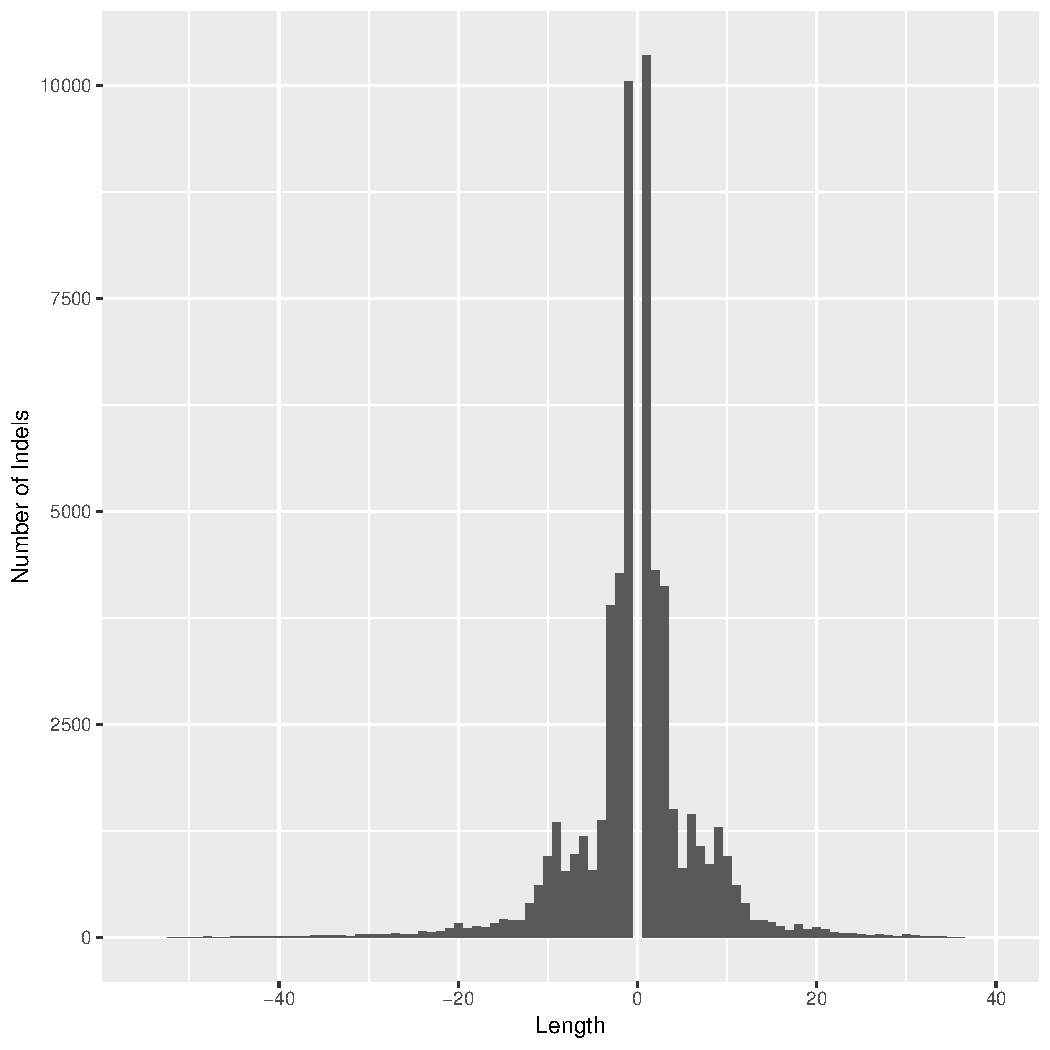
\includegraphics[angle=0,width=0.75\linewidth]{Figures/Ar109_histogram.pdf}}
		\resizebox{78mm}{78mm}{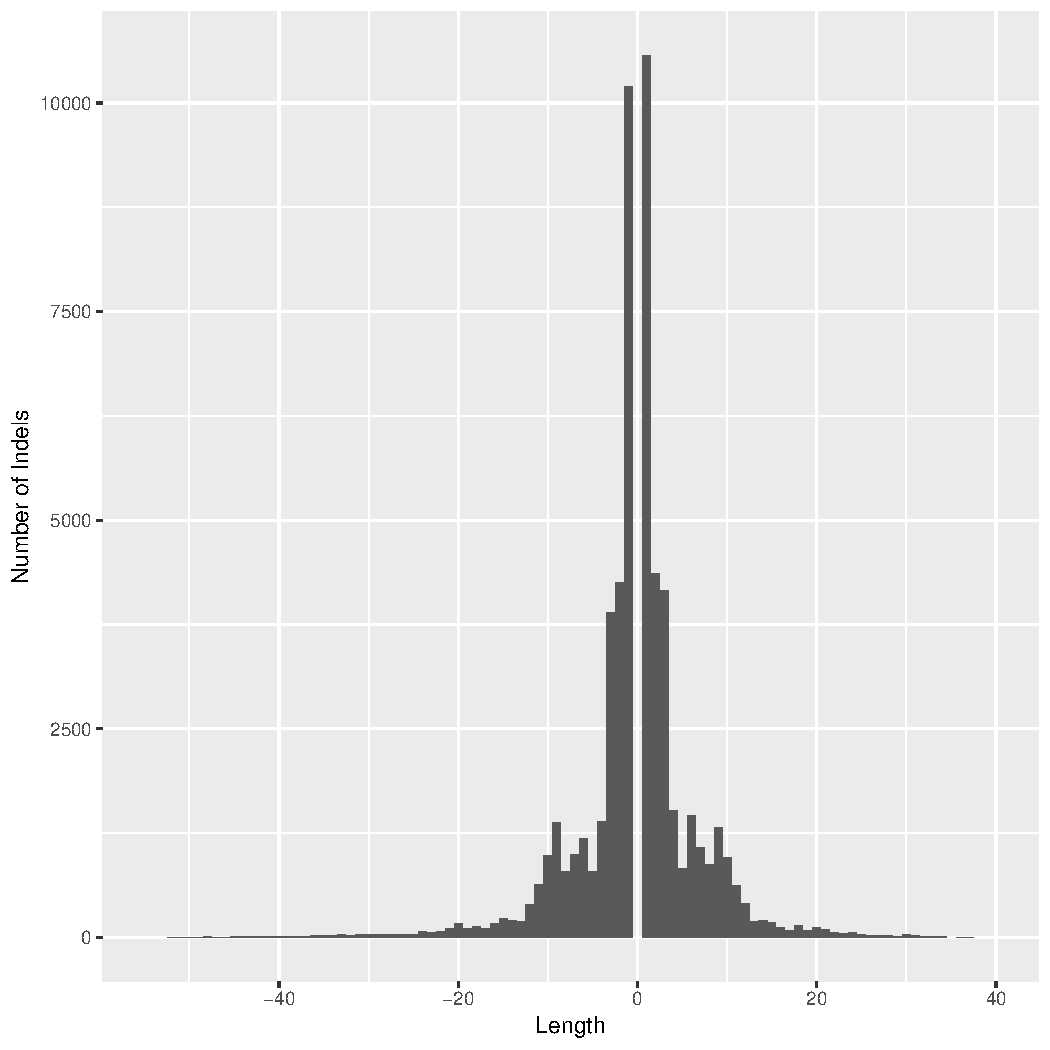
\includegraphics[angle=0,width=0.75\linewidth]{Figures/Ar119_histogram.pdf}}\\
		\resizebox{78mm}{78mm}{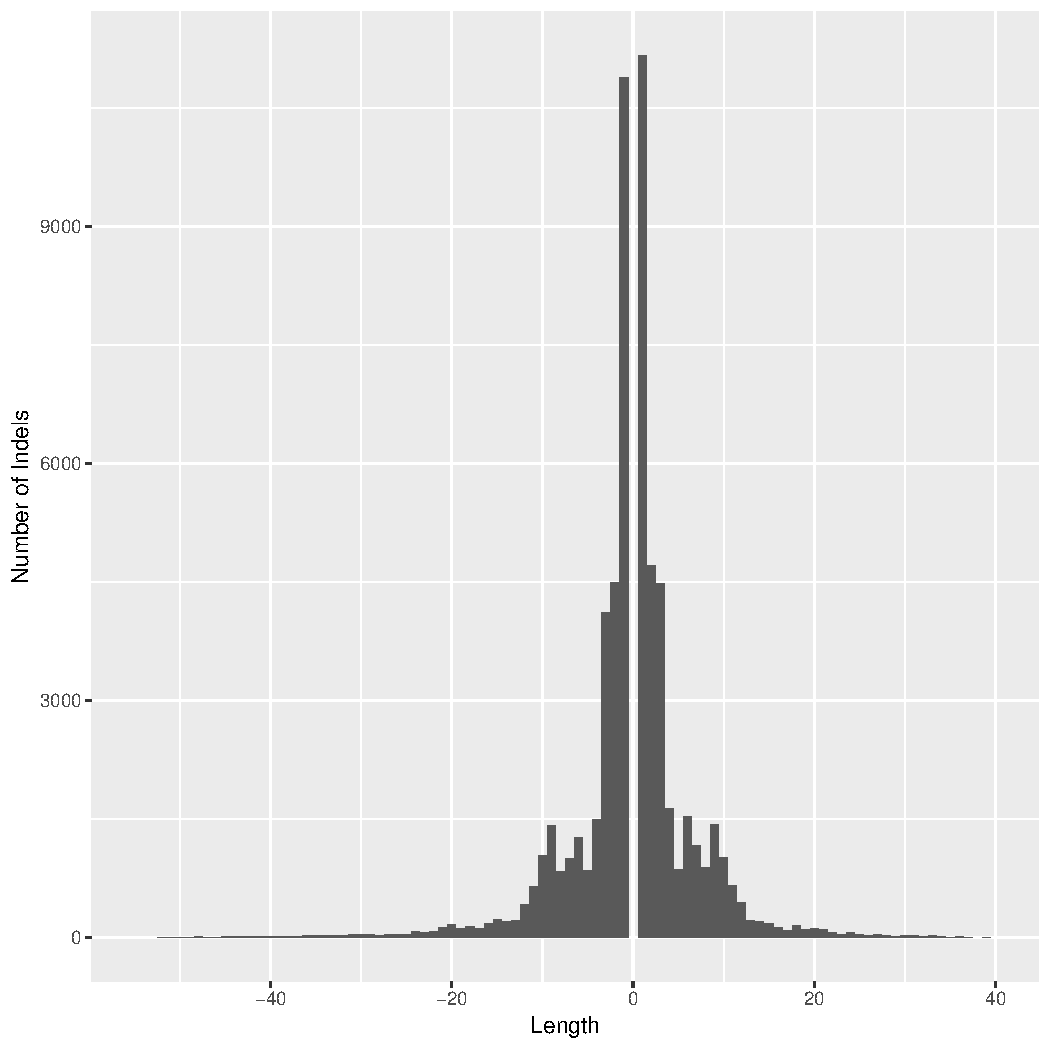
\includegraphics[angle=0,width=1.0\linewidth]{Figures/Ar142_histogram.pdf}}
		\resizebox{78mm}{78mm}{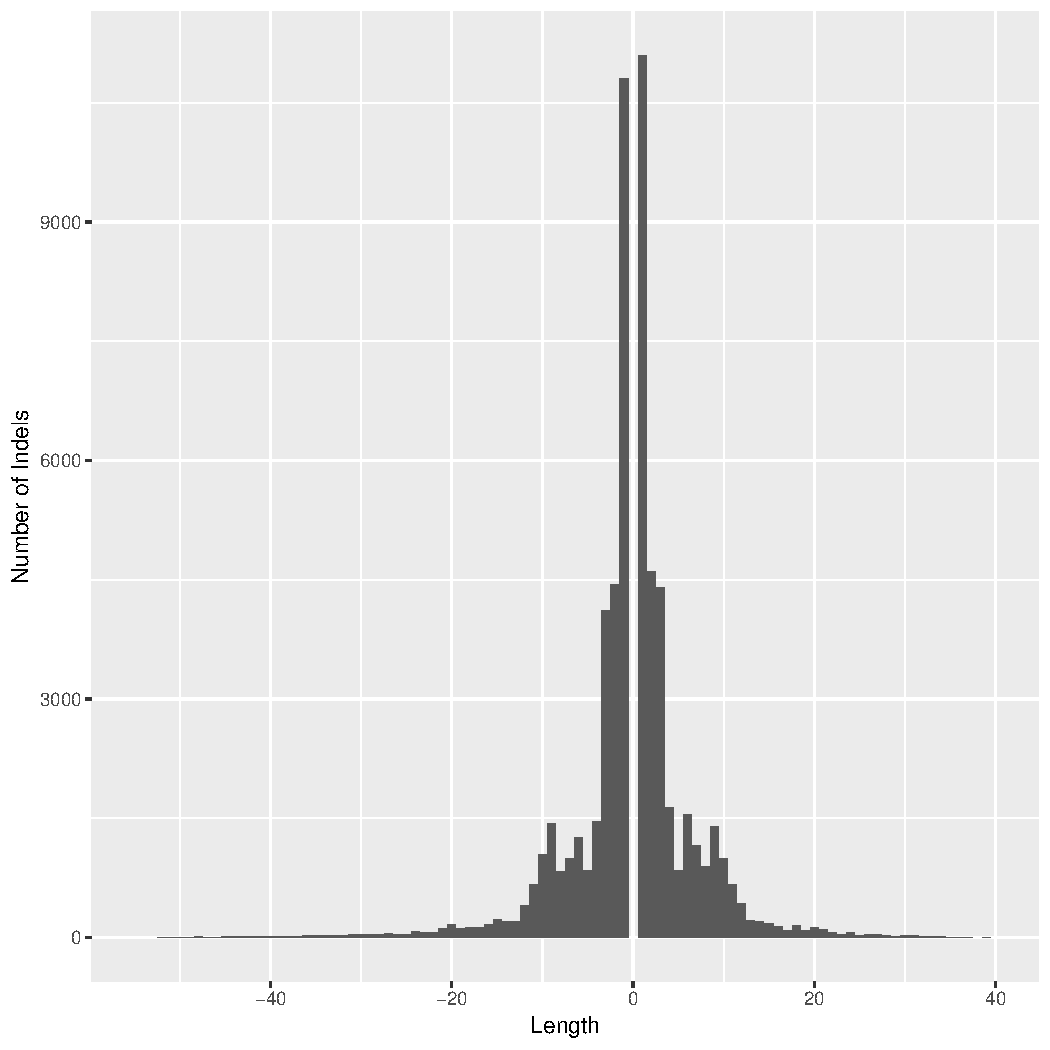
\includegraphics[angle=0,width=1.0\linewidth]{Figures/Ar159_histogram.pdf}}\\
		\resizebox{78mm}{78mm}{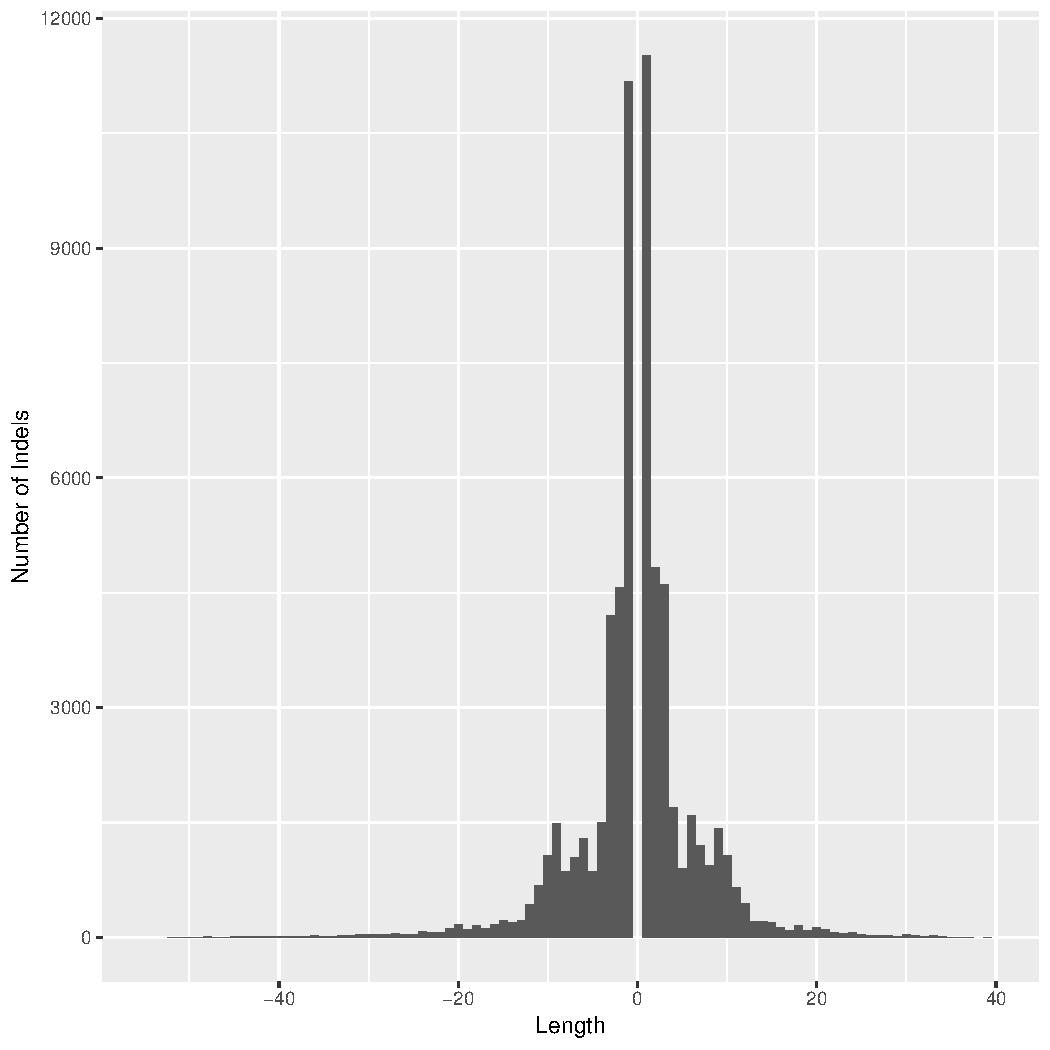
\includegraphics[angle=0,width=1.0\linewidth]{Figures/Ar170_histogram.pdf}}
		\resizebox{78mm}{78mm}{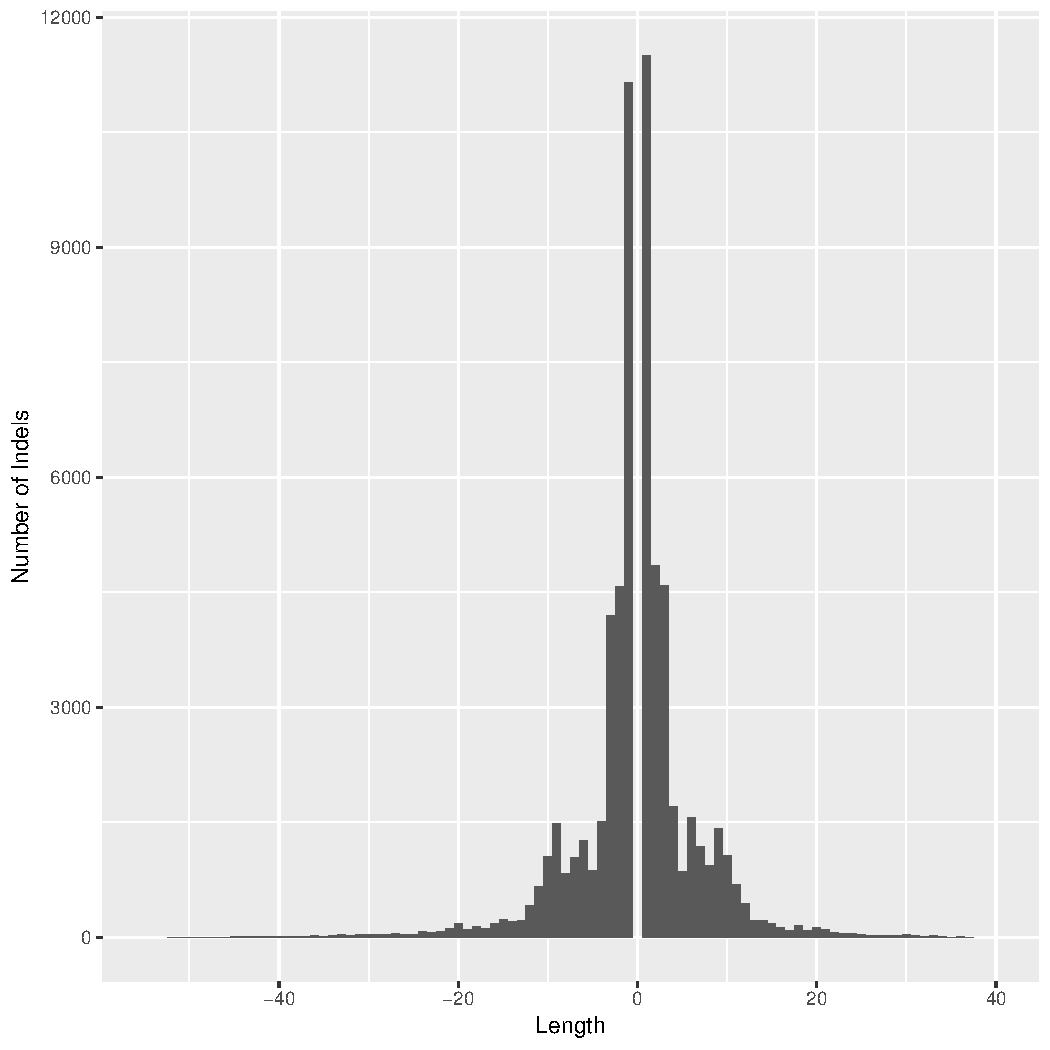
\includegraphics[angle=0,width=1.0\linewidth]{Figures/Ar174_histogram.pdf}}\\
		\begin{singlespace}
			\vspace{-0.5cm}
			\caption[The Frequency of the Indel Length]{The Frequency of the Indel Length Per Strain, Ar: 109, 119, 142, 159, 170, and 174}\label{Length_Indel_His}
		\end{singlespace}
	\end{centering}
\end{figure}

\begin{figure}[H]
	\begin{centering}
		\vspace{-1.5cm}
		\resizebox{78mm}{78mm}{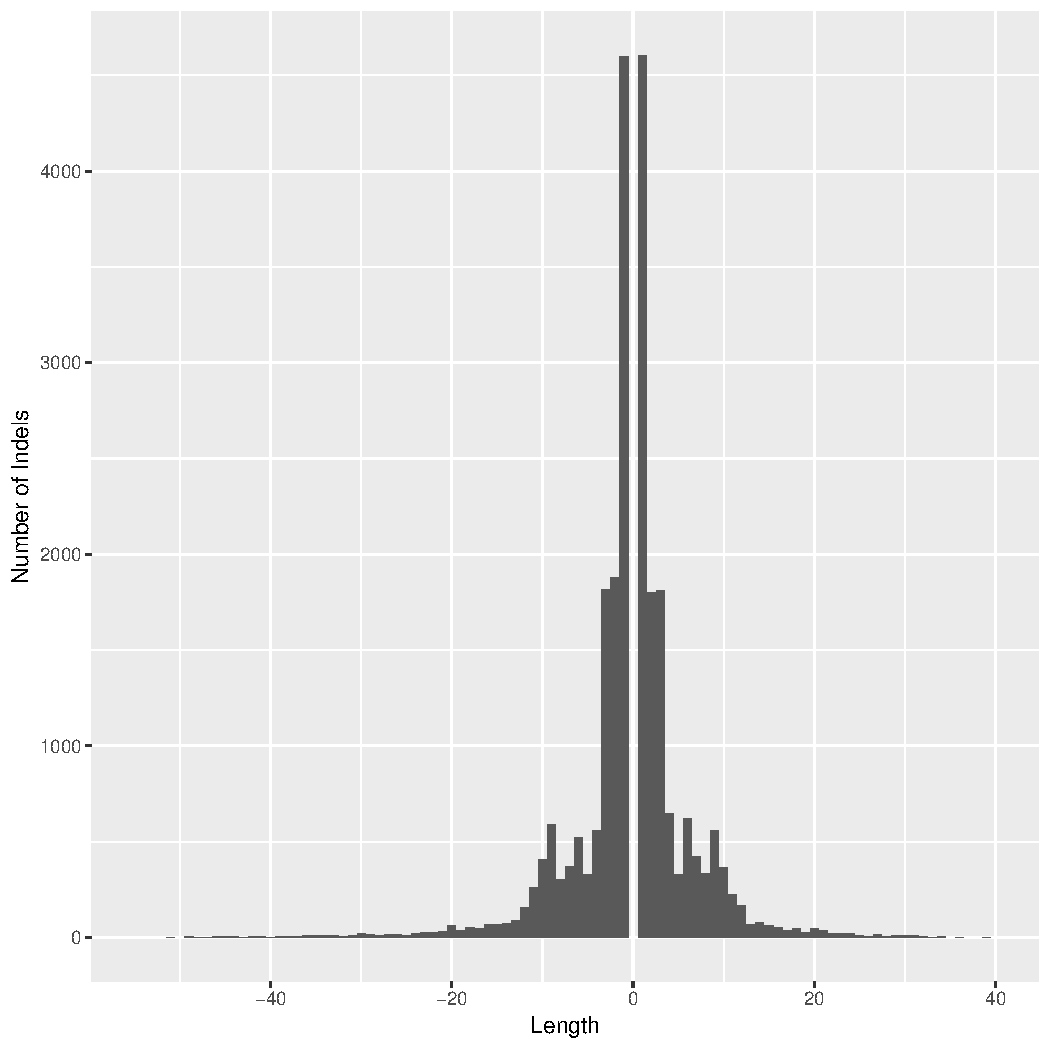
\includegraphics[angle=0,width=1.0\linewidth]{Figures/Ar175_histogram.pdf}}
		\resizebox{78mm}{78mm}{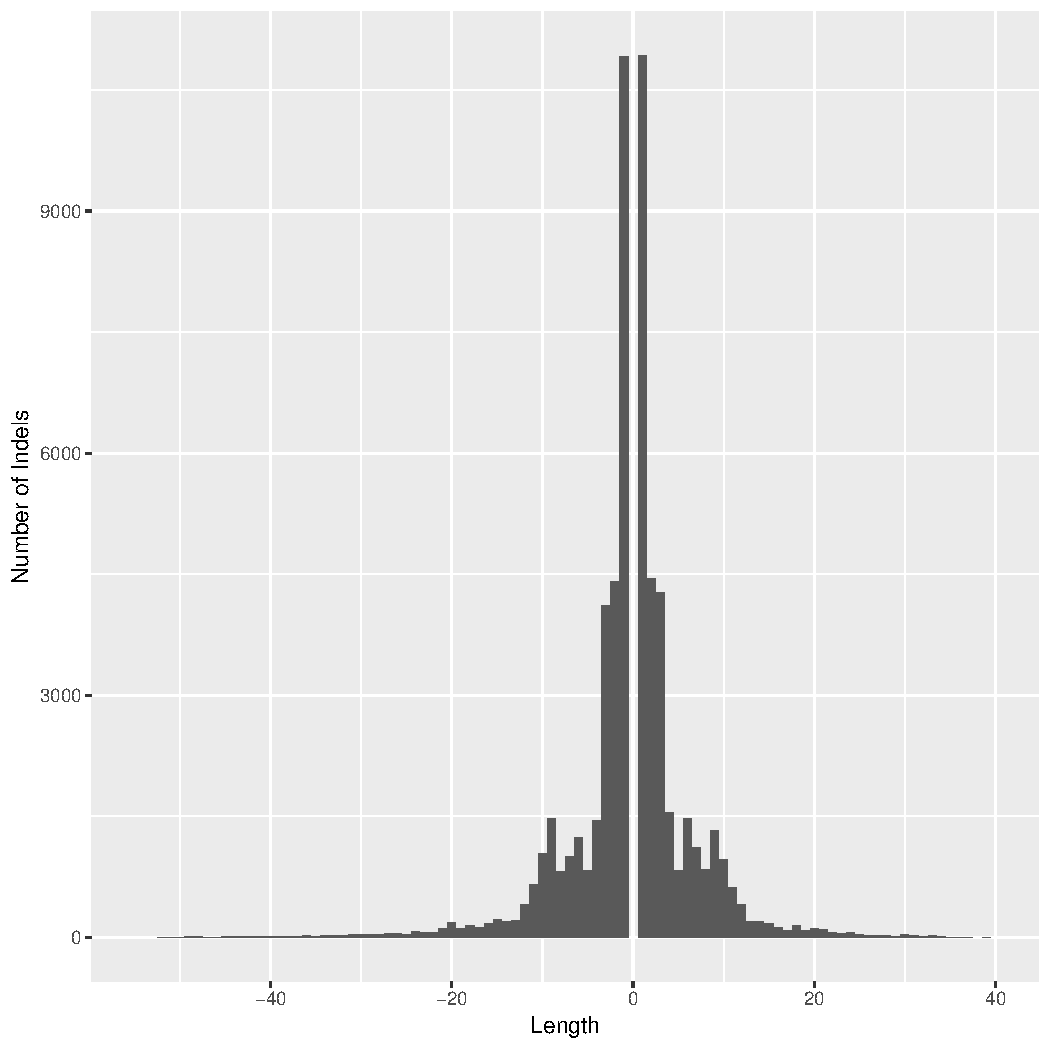
\includegraphics[angle=0,width=1.0\linewidth]{Figures/Ar176_histogram.pdf}}\\
		 \resizebox{78mm}{78mm}{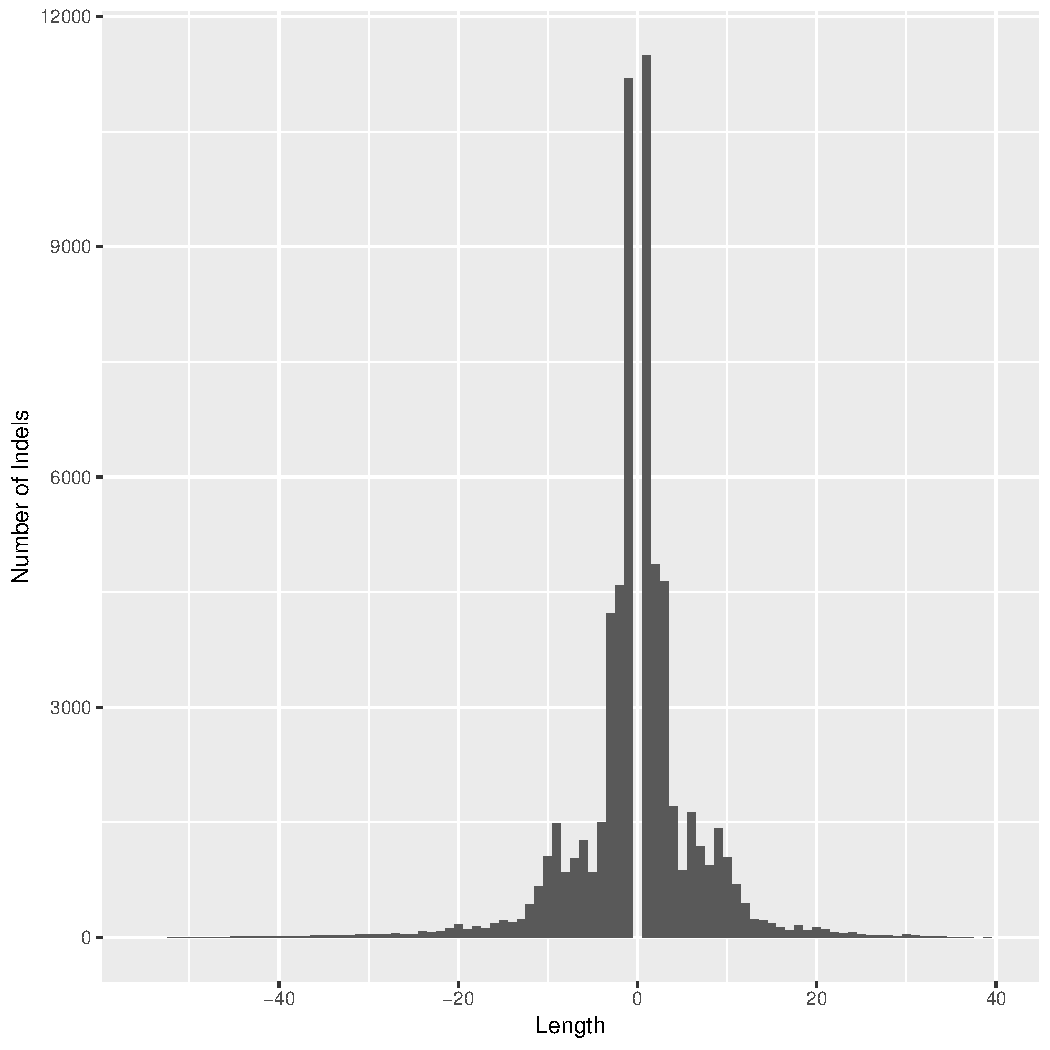
\includegraphics[angle=0,width=1.0\linewidth]{Figures/Ar179_histogram.pdf}}
		\resizebox{78mm}{78mm}{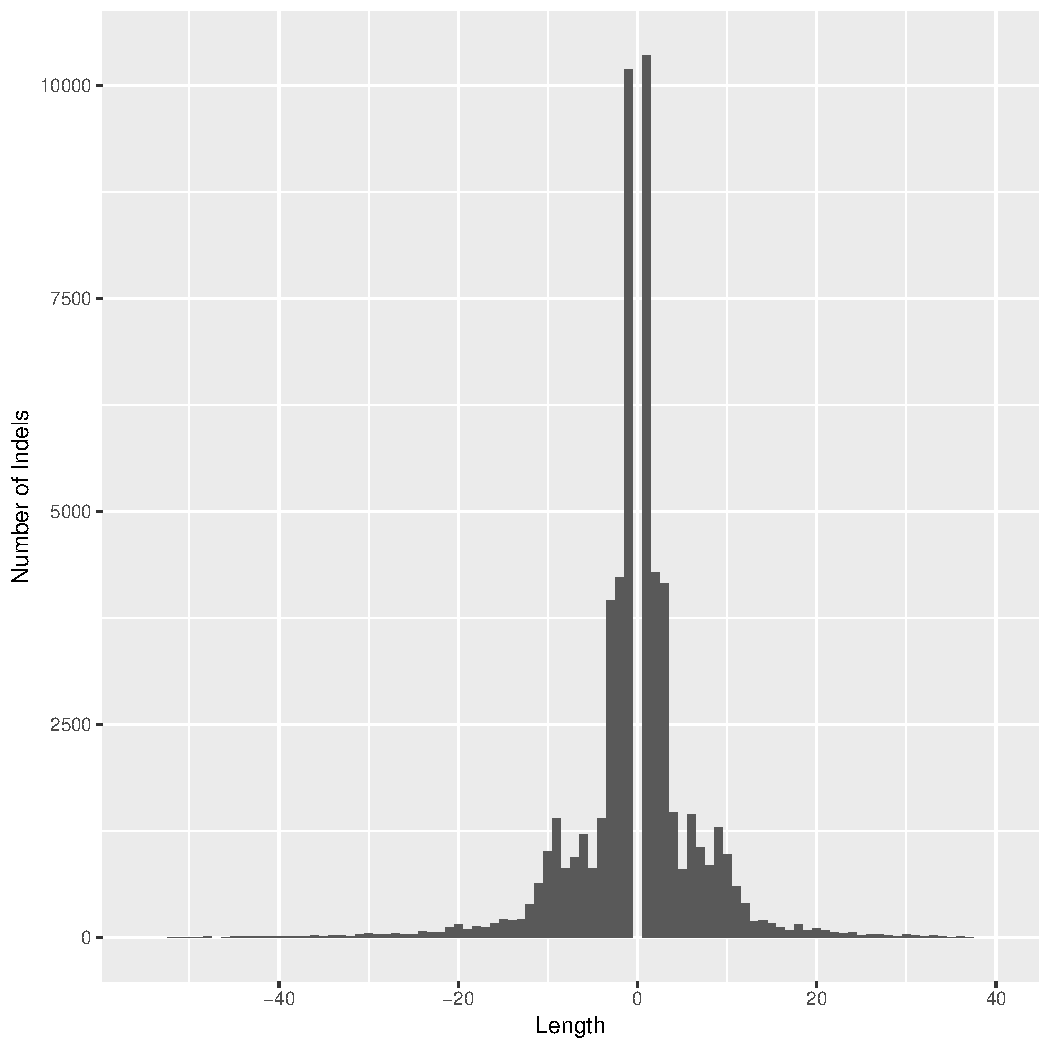
\includegraphics[angle=0,width=1.0\linewidth]{Figures/Ar188_histogram.pdf}}\\
		\resizebox{78mm}{78mm}{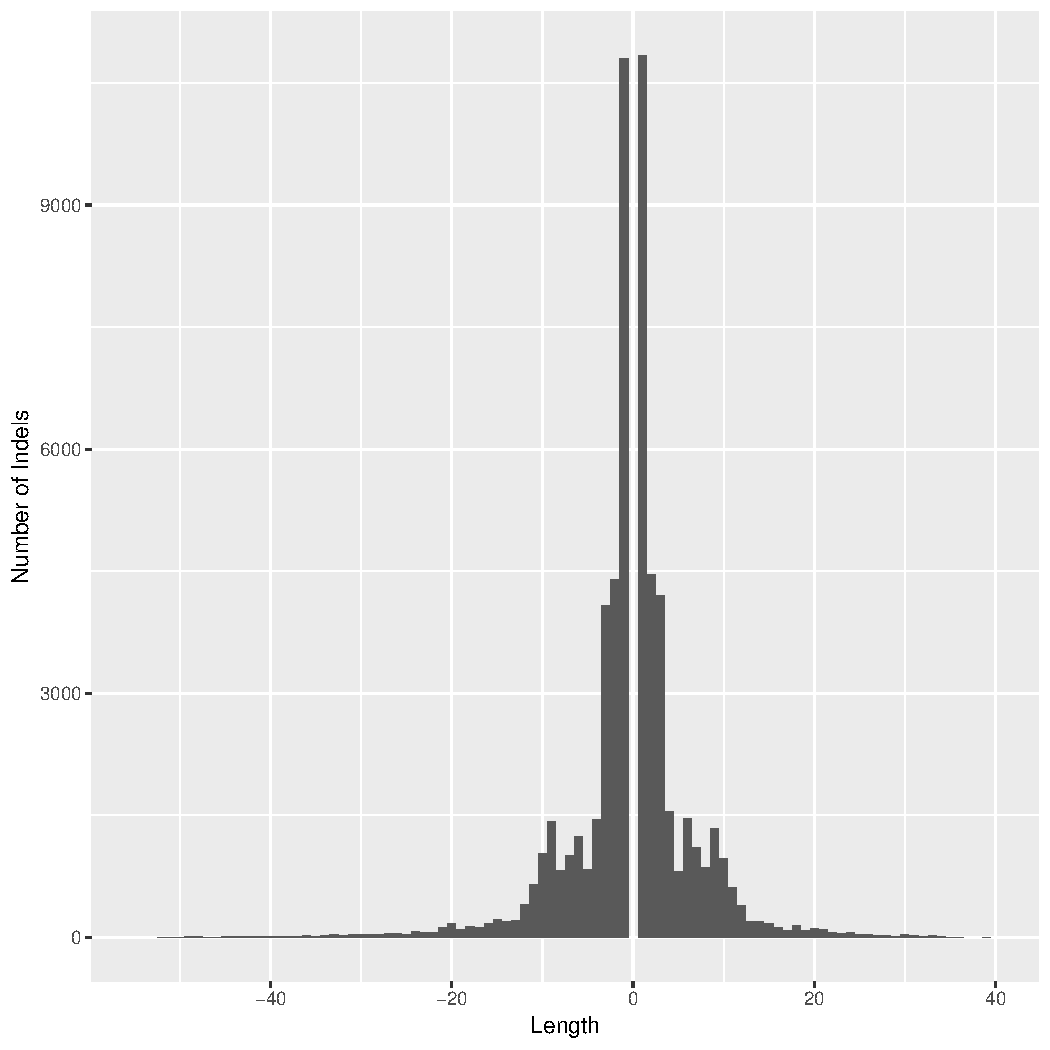
\includegraphics[angle=0,width=1.0\linewidth]{Figures/Ar194_histogram.pdf}}
		\resizebox{78mm}{78mm}{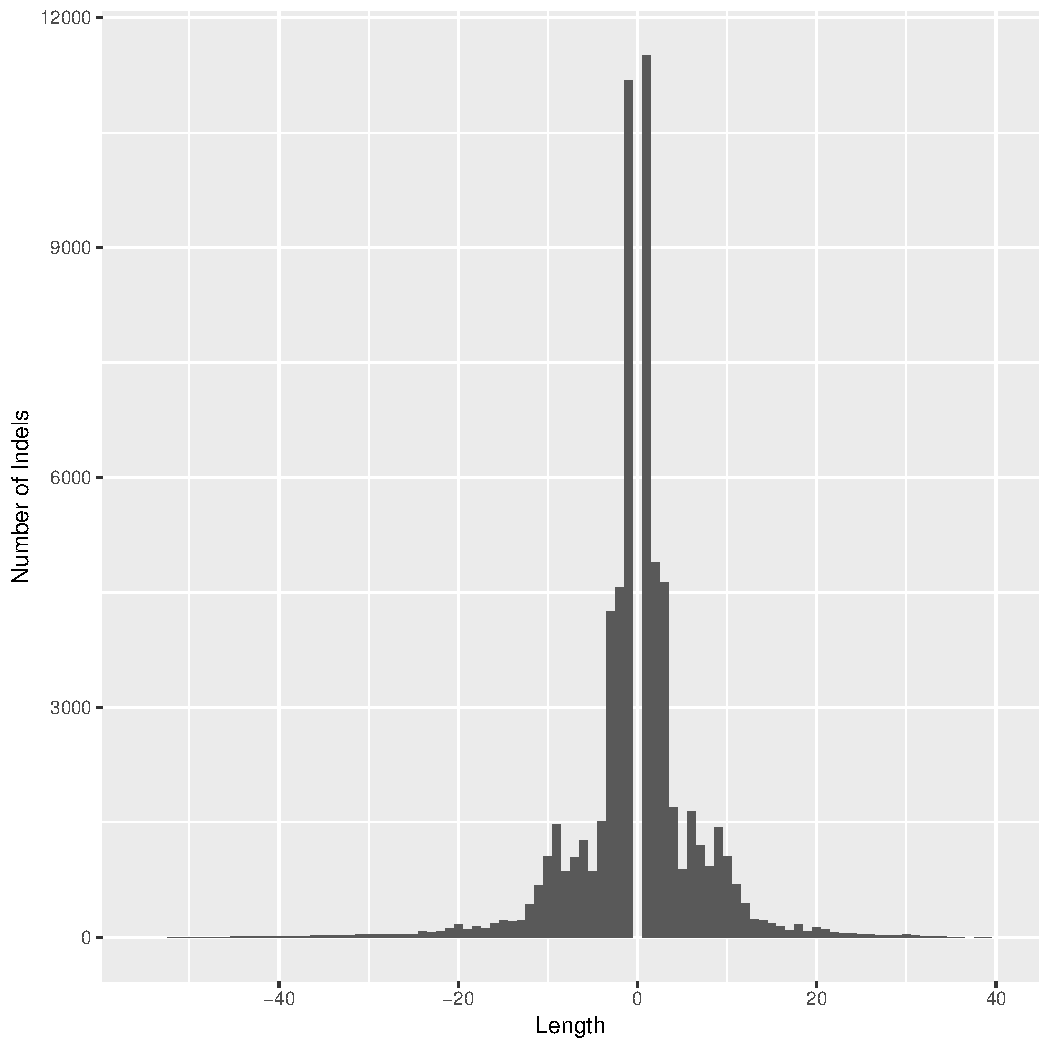
\includegraphics[angle=0,width=1.0\linewidth]{Figures/Ar196_histogram.pdf}}\\
		\begin{singlespace}
			\vspace{-0.5cm}
			\caption[The Frequency of the Indel Length2]{The Frequency of the Indel Length Per Strain, Ar: 175, 176, 179, 188, 194, and 196}\label{Length_Indel_His2}
		\end{singlespace}
	\end{centering}
\end{figure}

\begin{figure}[H]
	\begin{centering}
		\vspace{1.5cm}
                \resizebox{78mm}{78mm}{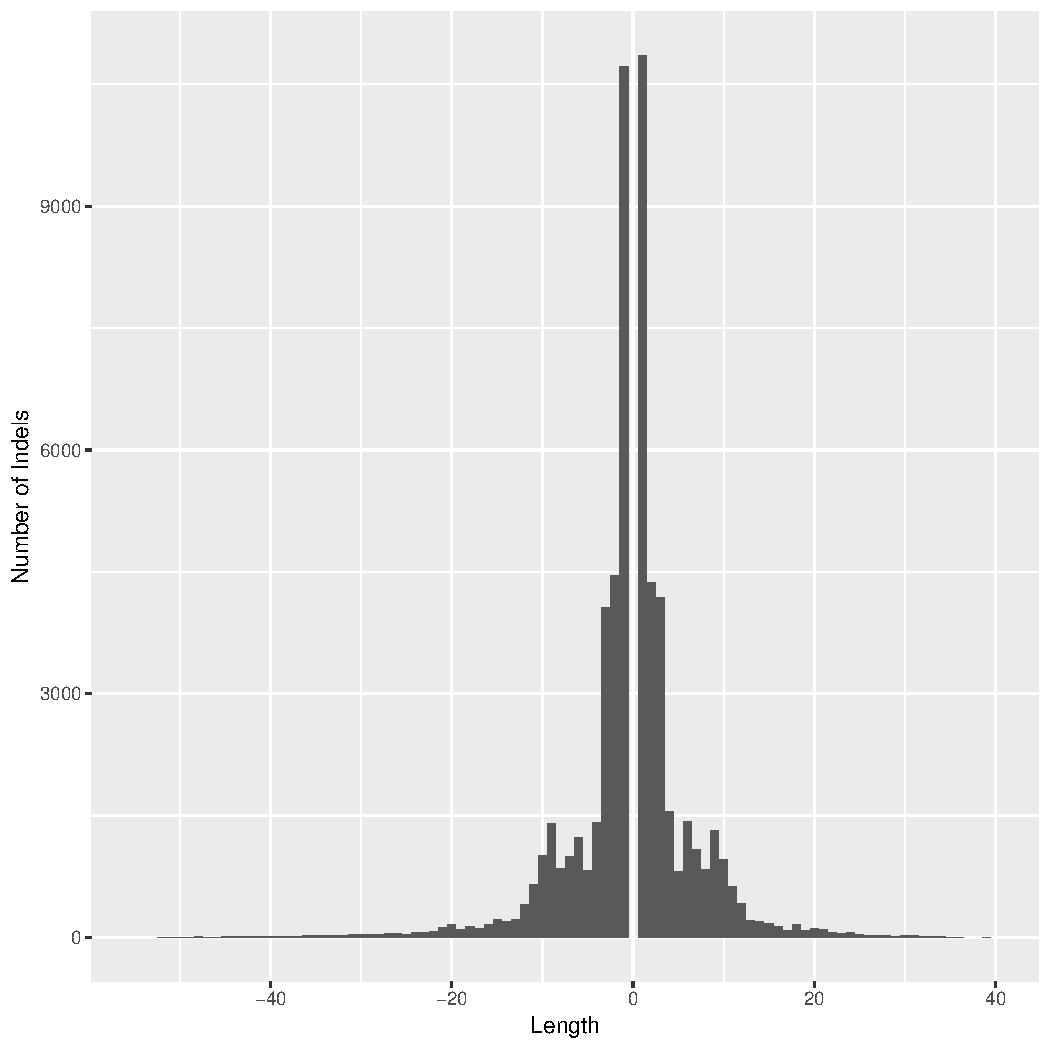
\includegraphics[angle=0,width=1.0\linewidth]{Figures/Ar201_histogram.pdf}}
		\resizebox{78mm}{78mm}{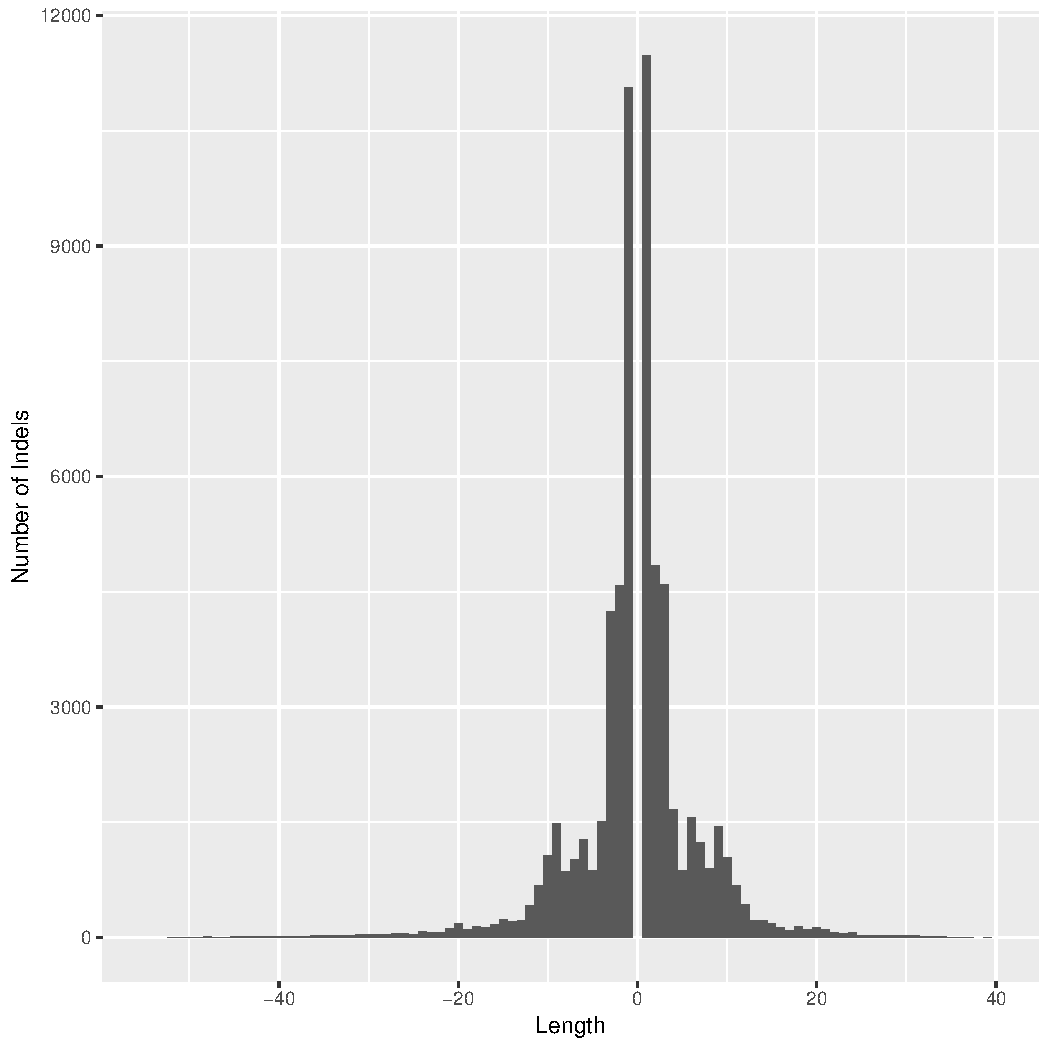
\includegraphics[angle=0,width=1.0\linewidth]{Figures/Ar213_histogram.pdf}}\\
		\resizebox{78mm}{78mm}{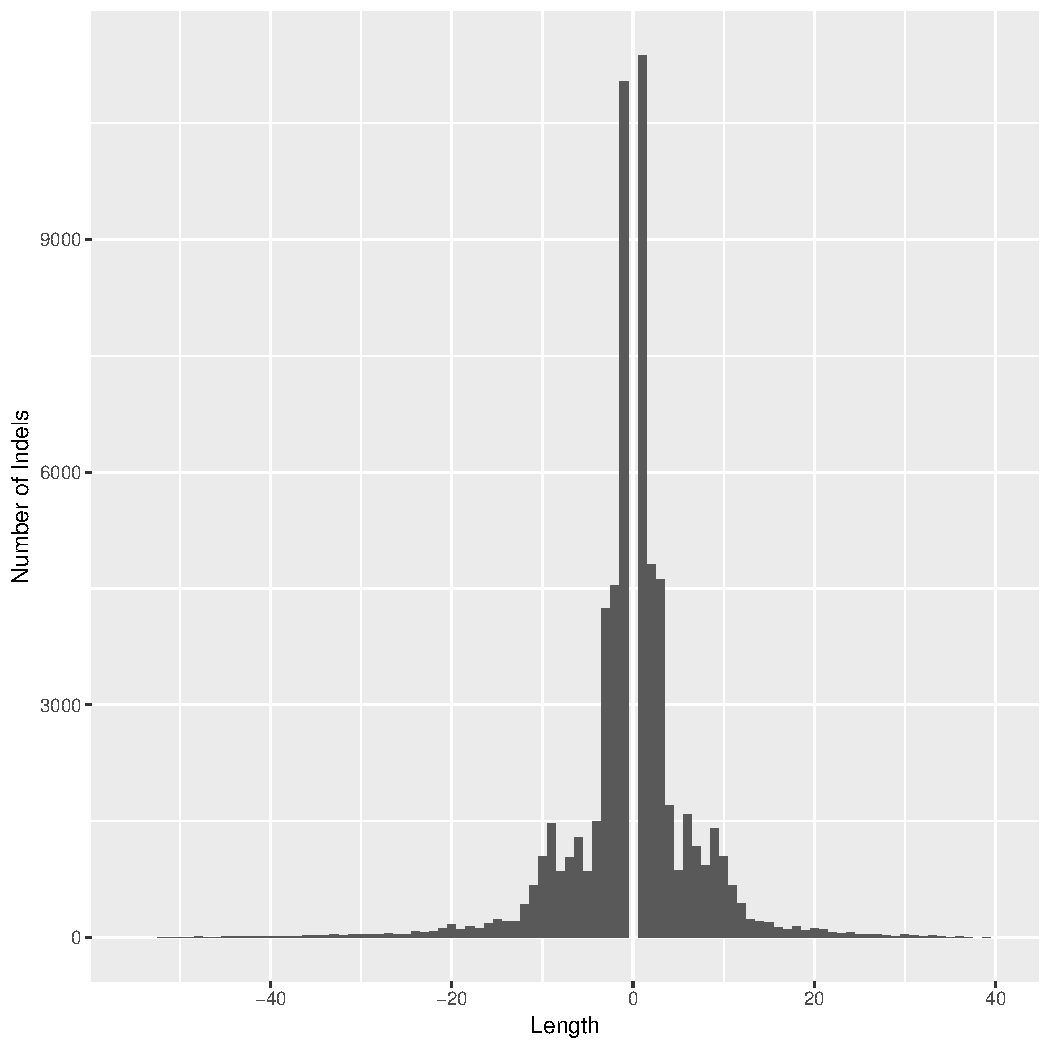
\includegraphics[angle=0,width=1.0\linewidth]{Figures/Ar73_histogram.pdf}}
		\begin{singlespace}
			 \vspace{-0.5cm}	
	\caption[The Frequency of the Indel Length3]{The Frequency of the Indel Length Per Strain, Ar: 201, 213, and73}\label{Length_Indel_His3}
		\end{singlespace}
	\end{centering}
\end{figure}
	

###FIX THESE###

\begin{figure}[H]
	\begin{centering}
		\vspace{1.5cm}
		\resizebox{78mm}{78mm}{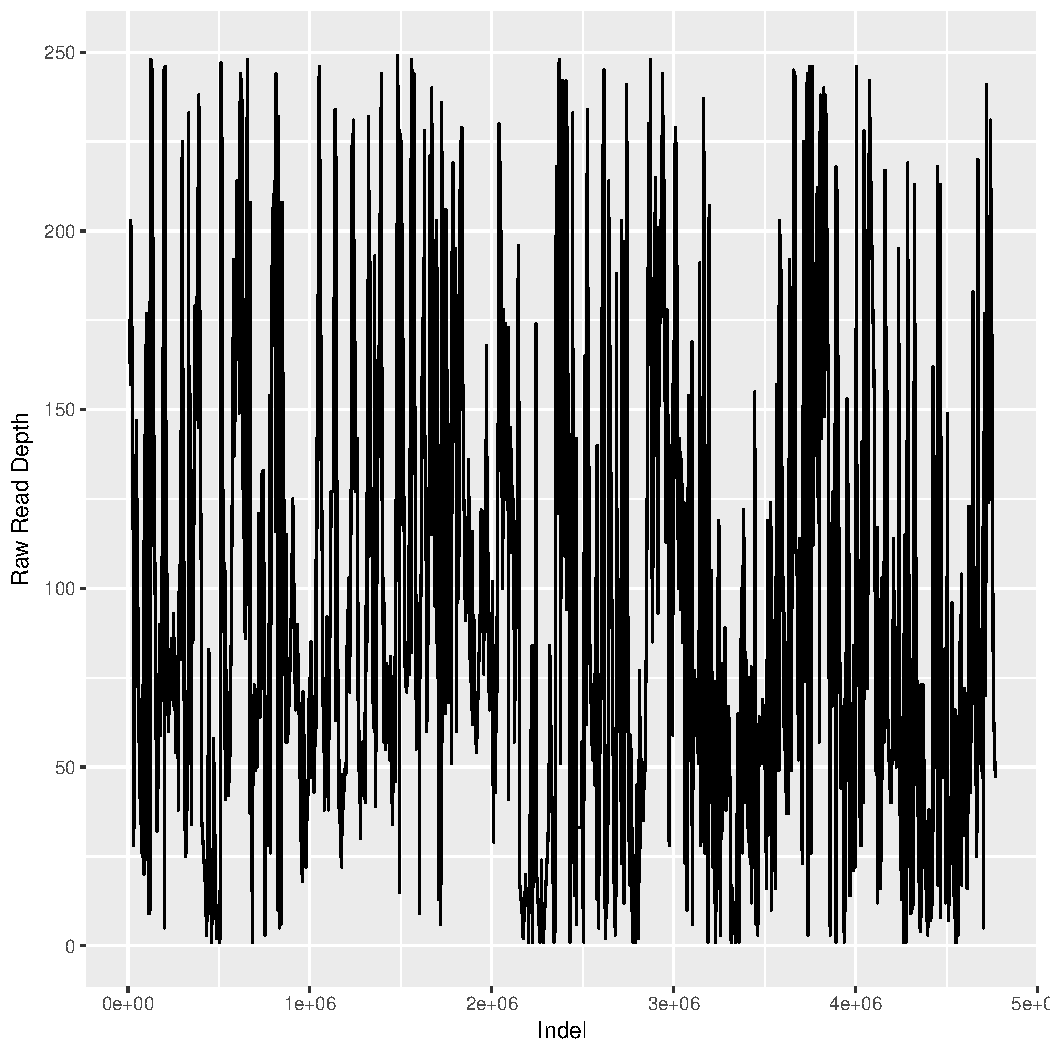
\includegraphics[angle=0,width=1.0\linewidth]{Figures/1_DP_locations.pdf}}
                \resizebox{78mm}{78mm}{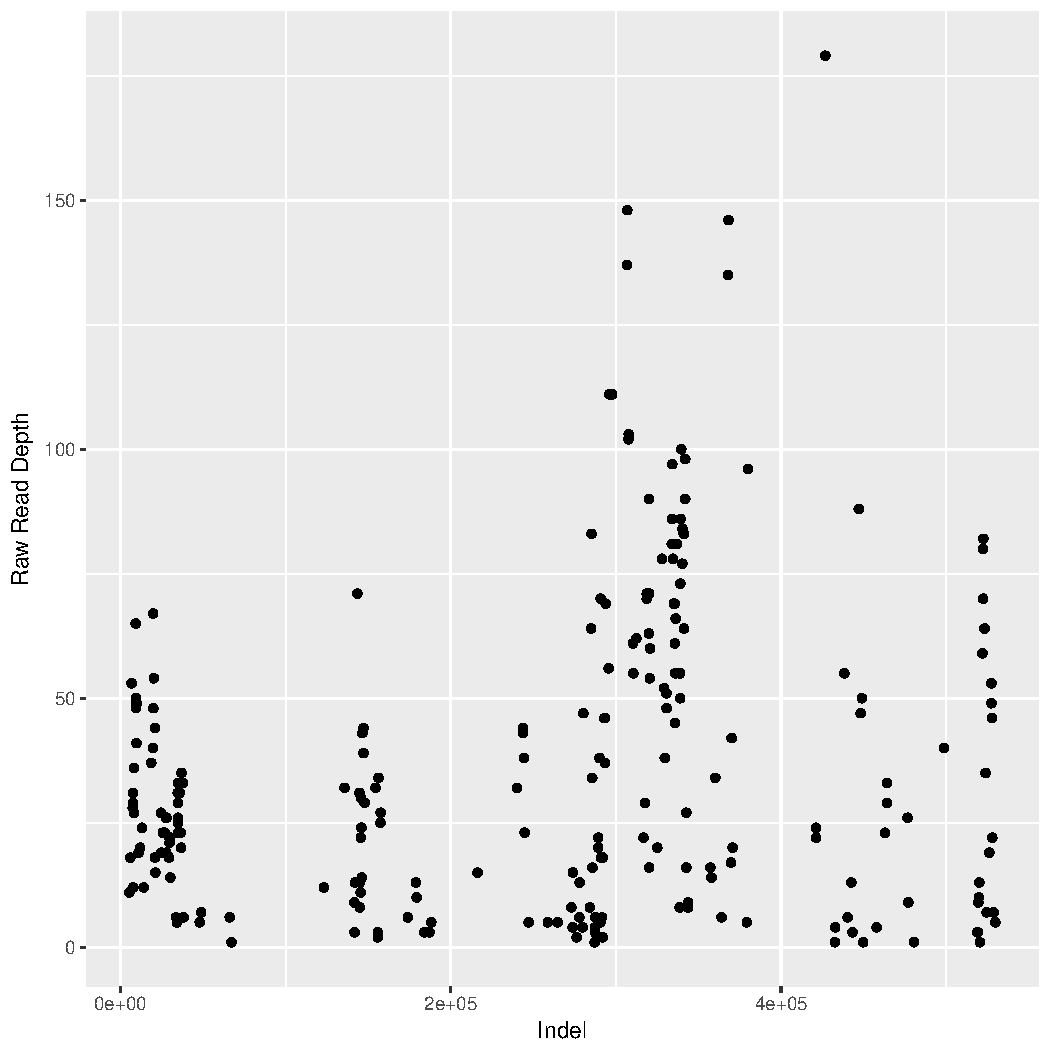
\includegraphics[angle=0,width=1.0\linewidth]{Figures/50_DP_locations.pdf}}\\
		\resizebox{78mm}{78mm}{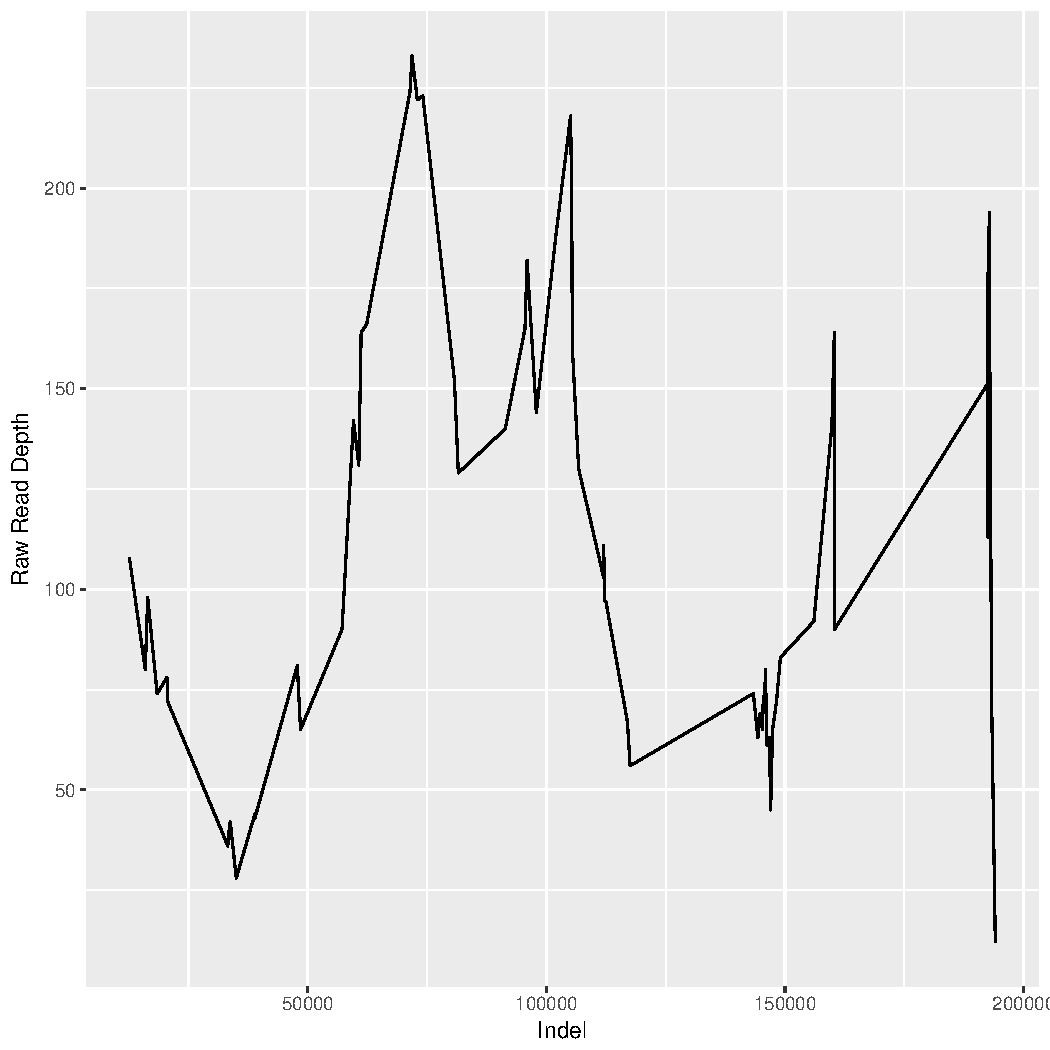
\includegraphics[angle=0,width=1.0\linewidth]{Figures/100_DP_locations.pdf}}
		\resizebox{78mm}{78mm}{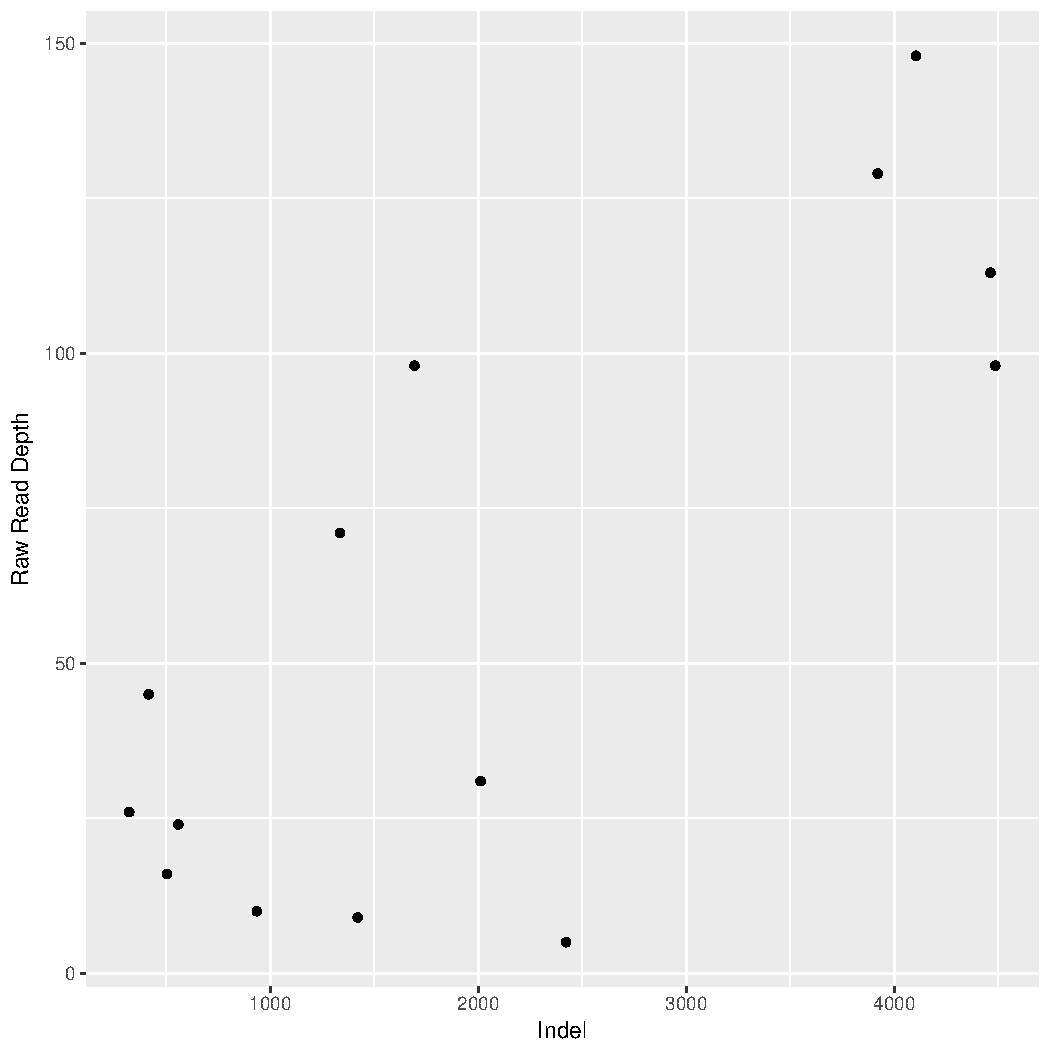
\includegraphics[angle=0,width=1.0\linewidth]{Figures/211_DP_locations.pdf}}
		\begin{singlespace}
		    \vspace{-0.5cm}	
		    \caption[The Read Depth of Indels Found]{The Read Depth of Indels Found in Ar:109 at Scaffold:1, 50, 100, and 211. Every vertice indicates one indel}\label{readdepth_indel}
	   \end{singlespace}
	\end{centering}
\end{figure}







\end{document}
